\documentclass[twoside]{book}

% Packages required by doxygen
\usepackage{calc}
\usepackage{doxygen}
\usepackage{graphicx}
\usepackage[utf8]{inputenc}
\usepackage{makeidx}
\usepackage{multicol}
\usepackage{multirow}
\usepackage{textcomp}
\usepackage[table]{xcolor}

% NLS support packages
\usepackage[french]{babel}

% Font selection
\usepackage[T1]{fontenc}
\usepackage{mathptmx}
\usepackage[scaled=.90]{helvet}
\usepackage{courier}
\usepackage{amssymb}
\usepackage{sectsty}
\renewcommand{\familydefault}{\sfdefault}
\allsectionsfont{%
  \fontseries{bc}\selectfont%
  \color{darkgray}%
}
\renewcommand{\DoxyLabelFont}{%
  \fontseries{bc}\selectfont%
  \color{darkgray}%
}

% Page & text layout
\usepackage{geometry}
\geometry{%
  a4paper,%
  top=2.5cm,%
  bottom=2.5cm,%
  left=2.5cm,%
  right=2.5cm%
}
\tolerance=750
\hfuzz=15pt
\hbadness=750
\setlength{\emergencystretch}{15pt}
\setlength{\parindent}{0cm}
\setlength{\parskip}{0.2cm}
\makeatletter
\renewcommand{\paragraph}{%
  \@startsection{paragraph}{4}{0ex}{-1.0ex}{1.0ex}{%
    \normalfont\normalsize\bfseries\SS@parafont%
  }%
}
\renewcommand{\subparagraph}{%
  \@startsection{subparagraph}{5}{0ex}{-1.0ex}{1.0ex}{%
    \normalfont\normalsize\bfseries\SS@subparafont%
  }%
}
\makeatother

% Headers & footers
\usepackage{fancyhdr}
\pagestyle{fancyplain}
\fancyhead[LE]{\fancyplain{}{\bfseries\thepage}}
\fancyhead[CE]{\fancyplain{}{}}
\fancyhead[RE]{\fancyplain{}{\bfseries\leftmark}}
\fancyhead[LO]{\fancyplain{}{\bfseries\rightmark}}
\fancyhead[CO]{\fancyplain{}{}}
\fancyhead[RO]{\fancyplain{}{\bfseries\thepage}}
\fancyfoot[LE]{\fancyplain{}{}}
\fancyfoot[CE]{\fancyplain{}{}}
\fancyfoot[RE]{\fancyplain{}{\bfseries\scriptsize Généré le Samedi 8 Mars 2014 17\-:40\-:20 pour Module de gestion d'erreur par Doxygen }}
\fancyfoot[LO]{\fancyplain{}{\bfseries\scriptsize Généré le Samedi 8 Mars 2014 17\-:40\-:20 pour Module de gestion d'erreur par Doxygen }}
\fancyfoot[CO]{\fancyplain{}{}}
\fancyfoot[RO]{\fancyplain{}{}}
\renewcommand{\footrulewidth}{0.4pt}
\renewcommand{\chaptermark}[1]{%
  \markboth{#1}{}%
}
\renewcommand{\sectionmark}[1]{%
  \markright{\thesection\ #1}%
}

% Indices & bibliography
\usepackage{natbib}
\usepackage[titles]{tocloft}
\setcounter{tocdepth}{3}
\setcounter{secnumdepth}{5}
\makeindex

% Hyperlinks (required, but should be loaded last)
\usepackage{ifpdf}
\ifpdf
  \usepackage[pdftex,pagebackref=true]{hyperref}
\else
  \usepackage[ps2pdf,pagebackref=true]{hyperref}
\fi
\hypersetup{%
  colorlinks=true,%
  linkcolor=blue,%
  citecolor=blue,%
  unicode%
}

% Custom commands
\newcommand{\clearemptydoublepage}{%
  \newpage{\pagestyle{empty}\cleardoublepage}%
}


%===== C O N T E N T S =====

\begin{document}

% Titlepage & ToC
\hypersetup{pageanchor=false}
\pagenumbering{roman}
\begin{titlepage}
\vspace*{7cm}
\begin{center}%
{\Large Module de gestion d'erreur \\[1ex]\large 1 }\\
\vspace*{1cm}
{\large Généré par Doxygen 1.8.6}\\
\vspace*{0.5cm}
{\small Samedi 8 Mars 2014 17:40:20}\\
\end{center}
\end{titlepage}
\clearemptydoublepage
\tableofcontents
\clearemptydoublepage
\pagenumbering{arabic}
\hypersetup{pageanchor=true}

%--- Begin generated contents ---
\chapter{Module d'erreurs}
\label{index}\hypertarget{index}{}Ce module a pour but d'écrire les erreurs dans un fichier \char`\"{}log.\-txt\char`\"{} afin d'en garder une trace si on veut les consulter.

{\bfseries Exemple de B\-O\-N\-N\-E utilisation du module \-: } \begin{DoxyVerb}  Log.error("l'erreur");
  Log.reset();\end{DoxyVerb}
 
\chapter{Index des espaces de nommage}
\section{Paquetages}
Liste des paquetages avec une brève description (si disponible) \-:\begin{DoxyCompactList}
\item\contentsline{section}{\hyperlink{namespacecom}{com} }{\pageref{d8/dee/namespacecom}}{}
\item\contentsline{section}{\hyperlink{namespacecom_1_1error__manager}{com.\-error\-\_\-manager} }{\pageref{d9/df7/namespacecom_1_1error__manager}}{}
\item\contentsline{section}{\hyperlink{namespacecom_1_1error__manager_1_1test}{com.\-error\-\_\-manager.\-test} }{\pageref{d5/d4b/namespacecom_1_1error__manager_1_1test}}{}
\end{DoxyCompactList}

\chapter{Index hiérarchique}
\section{Hiérarchie des classes}
Cette liste d'héritage est classée approximativement par ordre alphabétique \-:\begin{DoxyCompactList}
\item Applet\begin{DoxyCompactList}
\item \contentsline{section}{jnt.\-Bench.\-Applet}{\pageref{d7/ddf/classjnt_1_1Bench_1_1Applet}}{}
\end{DoxyCompactList}
\item \contentsline{section}{jnt.\-Bench\-Mark}{\pageref{d3/d2c/classjnt_1_1BenchMark}}{}
\item \contentsline{section}{jnt.\-Bench\-Mark\-Result}{\pageref{df/d04/classjnt_1_1BenchMarkResult}}{}
\item \contentsline{section}{jnt.\-Bench\-Mark\-Result\-Event}{\pageref{d3/dcf/interfacejnt_1_1BenchMarkResultEvent}}{}
\item \contentsline{section}{jnt.\-scimark2.\-Constants}{\pageref{d5/d9d/classjnt_1_1scimark2_1_1Constants}}{}
\item \contentsline{section}{jnt.\-scimark2.\-F\-F\-T}{\pageref{d2/d87/classjnt_1_1scimark2_1_1FFT}}{}
\item \contentsline{section}{jnt.\-Bench\-Mark\-Result.\-F\-F\-T}{\pageref{dd/d0a/classjnt_1_1BenchMarkResult_1_1FFT}}{}
\item \contentsline{section}{jnt.\-Bench.\-Formatter}{\pageref{d2/dcd/classjnt_1_1Bench_1_1Formatter}}{}
\item Frame\begin{DoxyCompactList}
\item \contentsline{section}{jnt.\-Bench.\-Submit\-Dialog}{\pageref{d0/da7/classjnt_1_1Bench_1_1SubmitDialog}}{}
\end{DoxyCompactList}
\item \contentsline{section}{jnt.\-Bench.\-H\-T\-T\-P\-Post}{\pageref{de/df0/classjnt_1_1Bench_1_1HTTPPost}}{}
\item \contentsline{section}{jnt.\-scimark2.\-Jacobi}{\pageref{d9/d30/classjnt_1_1scimark2_1_1Jacobi}}{}
\item \contentsline{section}{jnt.\-scimark2.\-kernel}{\pageref{d0/d13/classjnt_1_1scimark2_1_1kernel}}{}
\item \contentsline{section}{jnt.\-Bench\-Mark\-Result.\-L\-U}{\pageref{d6/dfb/classjnt_1_1BenchMarkResult_1_1LU}}{}
\item \contentsline{section}{jnt.\-scimark2.\-L\-U}{\pageref{d5/d6c/classjnt_1_1scimark2_1_1LU}}{}
\item \contentsline{section}{jnt.\-Bench\-Mark\-Result.\-Monte\-Carlo}{\pageref{d0/d37/classjnt_1_1BenchMarkResult_1_1MonteCarlo}}{}
\item \contentsline{section}{jnt.\-scimark2.\-Monte\-Carlo}{\pageref{dd/db2/classjnt_1_1scimark2_1_1MonteCarlo}}{}
\item \contentsline{section}{jnt.\-scimark2.\-Random}{\pageref{d0/d74/classjnt_1_1scimark2_1_1Random}}{}
\item Runnable\begin{DoxyCompactList}
\item \contentsline{section}{jnt.\-Bench.\-Bench}{\pageref{d1/d59/classjnt_1_1Bench_1_1Bench}}{}
\end{DoxyCompactList}
\item \contentsline{section}{jnt.\-Bench.\-Send\-Mail}{\pageref{d3/d4e/classjnt_1_1Bench_1_1SendMail}}{}
\item \contentsline{section}{jnt.\-Bench\-Mark\-Result.\-S\-O\-R}{\pageref{d8/dcd/classjnt_1_1BenchMarkResult_1_1SOR}}{}
\item \contentsline{section}{jnt.\-scimark2.\-S\-O\-R}{\pageref{d8/d38/classjnt_1_1scimark2_1_1SOR}}{}
\item \contentsline{section}{jnt.\-scimark2.\-Sparse\-Comp\-Row}{\pageref{db/dbd/classjnt_1_1scimark2_1_1SparseCompRow}}{}
\item \contentsline{section}{jnt.\-Bench\-Mark\-Result.\-Sparse\-Matmult}{\pageref{d5/ded/classjnt_1_1BenchMarkResult_1_1SparseMatmult}}{}
\item \contentsline{section}{jnt.\-scimark2.\-Stopwatch}{\pageref{d2/d17/classjnt_1_1scimark2_1_1Stopwatch}}{}
\item \contentsline{section}{jnt.\-Bench.\-Stopwatch}{\pageref{d9/d48/classjnt_1_1Bench_1_1Stopwatch}}{}
\item \contentsline{section}{jnt.\-Bench.\-Target}{\pageref{de/d37/interfacejnt_1_1Bench_1_1Target}}{}
\begin{DoxyCompactList}
\item \contentsline{section}{jnt.\-scimark2.\-applet}{\pageref{dd/dfe/classjnt_1_1scimark2_1_1applet}}{}
\end{DoxyCompactList}
\item Canvas\begin{DoxyCompactList}
\item \contentsline{section}{jnt.\-Bench.\-Plotter}{\pageref{da/d70/classjnt_1_1Bench_1_1Plotter}}{}
\end{DoxyCompactList}
\end{DoxyCompactList}

\chapter{Index des classes}
\section{Liste des classes}
Liste des classes, structures, unions et interfaces avec une brève description \-:\begin{DoxyCompactList}
\item\contentsline{section}{\hyperlink{classjnt_1_1Bench_1_1Applet}{jnt.\-Bench.\-Applet} }{\pageref{d7/ddf/classjnt_1_1Bench_1_1Applet}}{}
\item\contentsline{section}{\hyperlink{classjnt_1_1scimark2_1_1applet}{jnt.\-scimark2.\-applet} }{\pageref{dd/dfe/classjnt_1_1scimark2_1_1applet}}{}
\item\contentsline{section}{\hyperlink{classjnt_1_1Bench_1_1Bench}{jnt.\-Bench.\-Bench} }{\pageref{d1/d59/classjnt_1_1Bench_1_1Bench}}{}
\item\contentsline{section}{\hyperlink{classjnt_1_1BenchMark}{jnt.\-Bench\-Mark} }{\pageref{d3/d2c/classjnt_1_1BenchMark}}{}
\item\contentsline{section}{\hyperlink{classjnt_1_1BenchMarkResult}{jnt.\-Bench\-Mark\-Result} }{\pageref{df/d04/classjnt_1_1BenchMarkResult}}{}
\item\contentsline{section}{\hyperlink{interfacejnt_1_1BenchMarkResultEvent}{jnt.\-Bench\-Mark\-Result\-Event} }{\pageref{d3/dcf/interfacejnt_1_1BenchMarkResultEvent}}{}
\item\contentsline{section}{\hyperlink{classjnt_1_1scimark2_1_1Constants}{jnt.\-scimark2.\-Constants} }{\pageref{d5/d9d/classjnt_1_1scimark2_1_1Constants}}{}
\item\contentsline{section}{\hyperlink{classjnt_1_1scimark2_1_1FFT}{jnt.\-scimark2.\-F\-F\-T} }{\pageref{d2/d87/classjnt_1_1scimark2_1_1FFT}}{}
\item\contentsline{section}{\hyperlink{classjnt_1_1BenchMarkResult_1_1FFT}{jnt.\-Bench\-Mark\-Result.\-F\-F\-T} }{\pageref{dd/d0a/classjnt_1_1BenchMarkResult_1_1FFT}}{}
\item\contentsline{section}{\hyperlink{classjnt_1_1Bench_1_1Formatter}{jnt.\-Bench.\-Formatter} }{\pageref{d2/dcd/classjnt_1_1Bench_1_1Formatter}}{}
\item\contentsline{section}{\hyperlink{classjnt_1_1Bench_1_1HTTPPost}{jnt.\-Bench.\-H\-T\-T\-P\-Post} }{\pageref{de/df0/classjnt_1_1Bench_1_1HTTPPost}}{}
\item\contentsline{section}{\hyperlink{classjnt_1_1scimark2_1_1Jacobi}{jnt.\-scimark2.\-Jacobi} }{\pageref{d9/d30/classjnt_1_1scimark2_1_1Jacobi}}{}
\item\contentsline{section}{\hyperlink{classjnt_1_1scimark2_1_1kernel}{jnt.\-scimark2.\-kernel} }{\pageref{d0/d13/classjnt_1_1scimark2_1_1kernel}}{}
\item\contentsline{section}{\hyperlink{classjnt_1_1BenchMarkResult_1_1LU}{jnt.\-Bench\-Mark\-Result.\-L\-U} }{\pageref{d6/dfb/classjnt_1_1BenchMarkResult_1_1LU}}{}
\item\contentsline{section}{\hyperlink{classjnt_1_1scimark2_1_1LU}{jnt.\-scimark2.\-L\-U} }{\pageref{d5/d6c/classjnt_1_1scimark2_1_1LU}}{}
\item\contentsline{section}{\hyperlink{classjnt_1_1BenchMarkResult_1_1MonteCarlo}{jnt.\-Bench\-Mark\-Result.\-Monte\-Carlo} }{\pageref{d0/d37/classjnt_1_1BenchMarkResult_1_1MonteCarlo}}{}
\item\contentsline{section}{\hyperlink{classjnt_1_1scimark2_1_1MonteCarlo}{jnt.\-scimark2.\-Monte\-Carlo} }{\pageref{dd/db2/classjnt_1_1scimark2_1_1MonteCarlo}}{}
\item\contentsline{section}{\hyperlink{classjnt_1_1Bench_1_1Plotter}{jnt.\-Bench.\-Plotter} }{\pageref{da/d70/classjnt_1_1Bench_1_1Plotter}}{}
\item\contentsline{section}{\hyperlink{classjnt_1_1scimark2_1_1Random}{jnt.\-scimark2.\-Random} }{\pageref{d0/d74/classjnt_1_1scimark2_1_1Random}}{}
\item\contentsline{section}{\hyperlink{classjnt_1_1Bench_1_1SendMail}{jnt.\-Bench.\-Send\-Mail} }{\pageref{d3/d4e/classjnt_1_1Bench_1_1SendMail}}{}
\item\contentsline{section}{\hyperlink{classjnt_1_1BenchMarkResult_1_1SOR}{jnt.\-Bench\-Mark\-Result.\-S\-O\-R} }{\pageref{d8/dcd/classjnt_1_1BenchMarkResult_1_1SOR}}{}
\item\contentsline{section}{\hyperlink{classjnt_1_1scimark2_1_1SOR}{jnt.\-scimark2.\-S\-O\-R} }{\pageref{d8/d38/classjnt_1_1scimark2_1_1SOR}}{}
\item\contentsline{section}{\hyperlink{classjnt_1_1scimark2_1_1SparseCompRow}{jnt.\-scimark2.\-Sparse\-Comp\-Row} }{\pageref{db/dbd/classjnt_1_1scimark2_1_1SparseCompRow}}{}
\item\contentsline{section}{\hyperlink{classjnt_1_1BenchMarkResult_1_1SparseMatmult}{jnt.\-Bench\-Mark\-Result.\-Sparse\-Matmult} }{\pageref{d5/ded/classjnt_1_1BenchMarkResult_1_1SparseMatmult}}{}
\item\contentsline{section}{\hyperlink{classjnt_1_1scimark2_1_1Stopwatch}{jnt.\-scimark2.\-Stopwatch} }{\pageref{d2/d17/classjnt_1_1scimark2_1_1Stopwatch}}{}
\item\contentsline{section}{\hyperlink{classjnt_1_1Bench_1_1Stopwatch}{jnt.\-Bench.\-Stopwatch} }{\pageref{d9/d48/classjnt_1_1Bench_1_1Stopwatch}}{}
\item\contentsline{section}{\hyperlink{classjnt_1_1Bench_1_1SubmitDialog}{jnt.\-Bench.\-Submit\-Dialog} }{\pageref{d0/da7/classjnt_1_1Bench_1_1SubmitDialog}}{}
\item\contentsline{section}{\hyperlink{interfacejnt_1_1Bench_1_1Target}{jnt.\-Bench.\-Target} }{\pageref{de/d37/interfacejnt_1_1Bench_1_1Target}}{}
\end{DoxyCompactList}

\chapter{Index des fichiers}
\section{Liste des fichiers}
Liste de tous les fichiers avec une brève description \-:\begin{DoxyCompactList}
\item\contentsline{section}{\hyperlink{AllTests_8java}{All\-Tests.\-java} }{\pageref{d4/d12/AllTests_8java}}{}
\item\contentsline{section}{\hyperlink{Log_8java}{Log.\-java} }{\pageref{d4/d3d/Log_8java}}{}
\item\contentsline{section}{\hyperlink{LogTest_8java}{Log\-Test.\-java} }{\pageref{d2/d02/LogTest_8java}}{}
\end{DoxyCompactList}

\chapter{Documentation des espaces de nommage}
\hypertarget{namespacecom}{\section{Paquetage com}
\label{namespacecom}\index{com@{com}}
}
\subsection*{Paquetages}
\begin{DoxyCompactItemize}
\item 
package \hyperlink{namespacecom_1_1error__manager}{error\-\_\-manager}
\end{DoxyCompactItemize}

\hypertarget{namespacecom_1_1error__manager}{\section{Paquetage com.\-error\-\_\-manager}
\label{namespacecom_1_1error__manager}\index{com.\-error\-\_\-manager@{com.\-error\-\_\-manager}}
}
\subsection*{Paquetages}
\begin{DoxyCompactItemize}
\item 
package \hyperlink{namespacecom_1_1error__manager_1_1test}{test}
\end{DoxyCompactItemize}
\subsection*{Classes}
\begin{DoxyCompactItemize}
\item 
class \hyperlink{classcom_1_1error__manager_1_1Log}{Log}
\end{DoxyCompactItemize}

\hypertarget{namespacecom_1_1error__manager_1_1test}{\section{Paquetage com.\-error\-\_\-manager.\-test}
\label{namespacecom_1_1error__manager_1_1test}\index{com.\-error\-\_\-manager.\-test@{com.\-error\-\_\-manager.\-test}}
}
\subsection*{Classes}
\begin{DoxyCompactItemize}
\item 
class \hyperlink{classcom_1_1error__manager_1_1test_1_1AllTests}{All\-Tests}
\item 
class \hyperlink{classcom_1_1error__manager_1_1test_1_1LogTest}{Log\-Test}
\end{DoxyCompactItemize}

\chapter{Documentation des classes}
\hypertarget{classcom_1_1error__manager_1_1test_1_1AllTests}{\section{Référence de la classe com.\-error\-\_\-manager.\-test.\-All\-Tests}
\label{classcom_1_1error__manager_1_1test_1_1AllTests}\index{com.\-error\-\_\-manager.\-test.\-All\-Tests@{com.\-error\-\_\-manager.\-test.\-All\-Tests}}
}


La documentation de cette classe a été générée à partir du fichier suivant \-:\begin{DoxyCompactItemize}
\item 
\hyperlink{AllTests_8java}{All\-Tests.\-java}\end{DoxyCompactItemize}

\hypertarget{classcom_1_1error__manager_1_1Log}{\section{Référence de la classe com.\-error\-\_\-manager.\-Log}
\label{classcom_1_1error__manager_1_1Log}\index{com.\-error\-\_\-manager.\-Log@{com.\-error\-\_\-manager.\-Log}}
}
\subsection*{Fonctions membres publiques statiques}
\begin{DoxyCompactItemize}
\item 
static void \hyperlink{classcom_1_1error__manager_1_1Log_a166a04ee1ab46156746a99f2350103c6}{error} (String error)
\item 
static void \hyperlink{classcom_1_1error__manager_1_1Log_aec6d0b8d25d518ad666b2007fa7f6227}{reset} ()
\end{DoxyCompactItemize}
\subsection*{Attributs privés statiques}
\begin{DoxyCompactItemize}
\item 
static final String \hyperlink{classcom_1_1error__manager_1_1Log_a473629efcbd7c2b85456b8e80ab46cd3}{F\-I\-L\-E\-\_\-\-N\-A\-M\-E} = \char`\"{}log.\-txt\char`\"{}
\item 
static final String \hyperlink{classcom_1_1error__manager_1_1Log_ab7a0b23daad7f39e20de0dac67011b82}{E\-R\-R\-O\-R} = \char`\"{}Erreur lors de l'écriture dans le fichier d'erreur!\char`\"{}
\item 
static final String \hyperlink{classcom_1_1error__manager_1_1Log_a2b163327c26f9f62da88ef109f0300c3}{E\-R\-R\-O\-R\-\_\-\-F\-I\-L\-E\-\_\-\-N\-O\-T\-\_\-\-F\-O\-U\-N\-D} = \char`\"{}Le fichier demandé est introuvable!\char`\"{}
\end{DoxyCompactItemize}


\subsection{Description détaillée}
Classe qui contient les deux méthodes static qui permettent d'écrire et réinitialiser le fichier d'erreurs \begin{DoxyAuthor}{Auteur}

\begin{DoxyItemize}
\item Morgane Badré 
\item Vincent Wilmet 
\end{DoxyItemize}
\end{DoxyAuthor}
\begin{DoxyVersion}{Version}
1.\-0 
\end{DoxyVersion}


\subsection{Documentation des fonctions membres}
\hypertarget{classcom_1_1error__manager_1_1Log_a166a04ee1ab46156746a99f2350103c6}{\index{com\-::error\-\_\-manager\-::\-Log@{com\-::error\-\_\-manager\-::\-Log}!error@{error}}
\index{error@{error}!com::error_manager::Log@{com\-::error\-\_\-manager\-::\-Log}}
\subsubsection[{error}]{\setlength{\rightskip}{0pt plus 5cm}static void com.\-error\-\_\-manager.\-Log.\-error (
\begin{DoxyParamCaption}
\item[{String}]{error}
\end{DoxyParamCaption}
)\hspace{0.3cm}{\ttfamily [static]}}}\label{classcom_1_1error__manager_1_1Log_a166a04ee1ab46156746a99f2350103c6}
Ecrit dans le fichier en sortie le texte entré en paramètre 
\begin{DoxyParams}{Paramètres}
{\em error} & La chaîne de caractères contenant l'erreur à écrire dans le fichier \\
\hline
\end{DoxyParams}
\hypertarget{classcom_1_1error__manager_1_1Log_aec6d0b8d25d518ad666b2007fa7f6227}{\index{com\-::error\-\_\-manager\-::\-Log@{com\-::error\-\_\-manager\-::\-Log}!reset@{reset}}
\index{reset@{reset}!com::error_manager::Log@{com\-::error\-\_\-manager\-::\-Log}}
\subsubsection[{reset}]{\setlength{\rightskip}{0pt plus 5cm}static void com.\-error\-\_\-manager.\-Log.\-reset (
\begin{DoxyParamCaption}
{}
\end{DoxyParamCaption}
)\hspace{0.3cm}{\ttfamily [static]}}}\label{classcom_1_1error__manager_1_1Log_aec6d0b8d25d518ad666b2007fa7f6227}
Méthode réinitialisant le fichier d'erreur \par
 {\bfseries Attention \-: } Cette méthode supprime complètement le contenu du fichier 

\subsection{Documentation des données membres}
\hypertarget{classcom_1_1error__manager_1_1Log_ab7a0b23daad7f39e20de0dac67011b82}{\index{com\-::error\-\_\-manager\-::\-Log@{com\-::error\-\_\-manager\-::\-Log}!E\-R\-R\-O\-R@{E\-R\-R\-O\-R}}
\index{E\-R\-R\-O\-R@{E\-R\-R\-O\-R}!com::error_manager::Log@{com\-::error\-\_\-manager\-::\-Log}}
\subsubsection[{E\-R\-R\-O\-R}]{\setlength{\rightskip}{0pt plus 5cm}final String com.\-error\-\_\-manager.\-Log.\-E\-R\-R\-O\-R = \char`\"{}Erreur lors de l'écriture dans le fichier d'erreur!\char`\"{}\hspace{0.3cm}{\ttfamily [static]}, {\ttfamily [private]}}}\label{classcom_1_1error__manager_1_1Log_ab7a0b23daad7f39e20de0dac67011b82}
Variable contenant le message affiché dans la sortie d'erreur en cas d'échec \hypertarget{classcom_1_1error__manager_1_1Log_a2b163327c26f9f62da88ef109f0300c3}{\index{com\-::error\-\_\-manager\-::\-Log@{com\-::error\-\_\-manager\-::\-Log}!E\-R\-R\-O\-R\-\_\-\-F\-I\-L\-E\-\_\-\-N\-O\-T\-\_\-\-F\-O\-U\-N\-D@{E\-R\-R\-O\-R\-\_\-\-F\-I\-L\-E\-\_\-\-N\-O\-T\-\_\-\-F\-O\-U\-N\-D}}
\index{E\-R\-R\-O\-R\-\_\-\-F\-I\-L\-E\-\_\-\-N\-O\-T\-\_\-\-F\-O\-U\-N\-D@{E\-R\-R\-O\-R\-\_\-\-F\-I\-L\-E\-\_\-\-N\-O\-T\-\_\-\-F\-O\-U\-N\-D}!com::error_manager::Log@{com\-::error\-\_\-manager\-::\-Log}}
\subsubsection[{E\-R\-R\-O\-R\-\_\-\-F\-I\-L\-E\-\_\-\-N\-O\-T\-\_\-\-F\-O\-U\-N\-D}]{\setlength{\rightskip}{0pt plus 5cm}final String com.\-error\-\_\-manager.\-Log.\-E\-R\-R\-O\-R\-\_\-\-F\-I\-L\-E\-\_\-\-N\-O\-T\-\_\-\-F\-O\-U\-N\-D = \char`\"{}Le fichier demandé est introuvable!\char`\"{}\hspace{0.3cm}{\ttfamily [static]}, {\ttfamily [private]}}}\label{classcom_1_1error__manager_1_1Log_a2b163327c26f9f62da88ef109f0300c3}
Variable contenant le message à afficher dans la sortie d'erreur si le fichier cible est introuvable \hypertarget{classcom_1_1error__manager_1_1Log_a473629efcbd7c2b85456b8e80ab46cd3}{\index{com\-::error\-\_\-manager\-::\-Log@{com\-::error\-\_\-manager\-::\-Log}!F\-I\-L\-E\-\_\-\-N\-A\-M\-E@{F\-I\-L\-E\-\_\-\-N\-A\-M\-E}}
\index{F\-I\-L\-E\-\_\-\-N\-A\-M\-E@{F\-I\-L\-E\-\_\-\-N\-A\-M\-E}!com::error_manager::Log@{com\-::error\-\_\-manager\-::\-Log}}
\subsubsection[{F\-I\-L\-E\-\_\-\-N\-A\-M\-E}]{\setlength{\rightskip}{0pt plus 5cm}final String com.\-error\-\_\-manager.\-Log.\-F\-I\-L\-E\-\_\-\-N\-A\-M\-E = \char`\"{}log.\-txt\char`\"{}\hspace{0.3cm}{\ttfamily [static]}, {\ttfamily [private]}}}\label{classcom_1_1error__manager_1_1Log_a473629efcbd7c2b85456b8e80ab46cd3}
Variable contenant le nom du fichier où l'on va écrire les erreurs 

La documentation de cette classe a été générée à partir du fichier suivant \-:\begin{DoxyCompactItemize}
\item 
\hyperlink{Log_8java}{Log.\-java}\end{DoxyCompactItemize}

\hypertarget{classcom_1_1error__manager_1_1test_1_1LogTest}{\section{Référence de la classe com.\-error\-\_\-manager.\-test.\-Log\-Test}
\label{classcom_1_1error__manager_1_1test_1_1LogTest}\index{com.\-error\-\_\-manager.\-test.\-Log\-Test@{com.\-error\-\_\-manager.\-test.\-Log\-Test}}
}
Graphe d'héritage de com.\-error\-\_\-manager.\-test.\-Log\-Test\-:\begin{figure}[H]
\begin{center}
\leavevmode
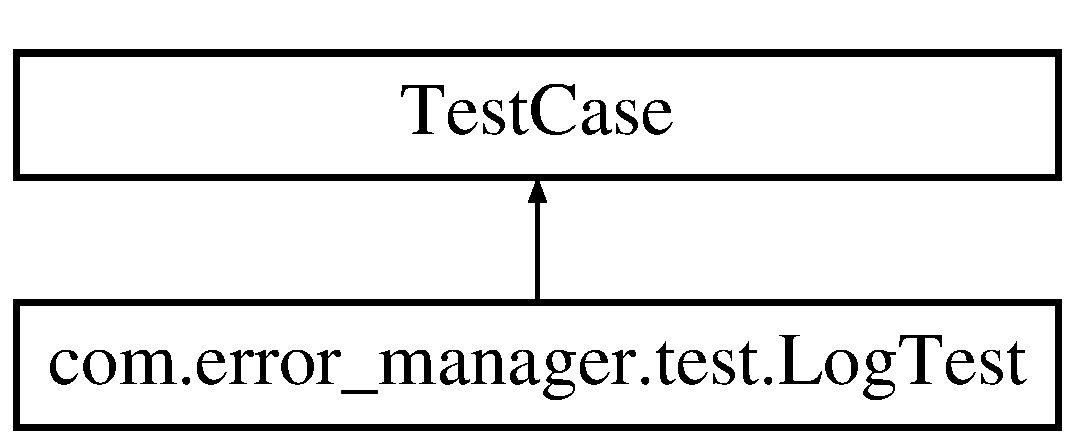
\includegraphics[height=2.000000cm]{d2/d45/classcom_1_1error__manager_1_1test_1_1LogTest}
\end{center}
\end{figure}
\subsection*{Fonctions membres publiques}
\begin{DoxyCompactItemize}
\item 
void \hyperlink{classcom_1_1error__manager_1_1test_1_1LogTest_a8a5ab3454826acbf2a7aa8bde0e66702}{test\-Error} ()
\item 
void \hyperlink{classcom_1_1error__manager_1_1test_1_1LogTest_a948eff44525b535e905756c1b66008c7}{test\-Reset} ()
\end{DoxyCompactItemize}


\subsection{Documentation des fonctions membres}
\hypertarget{classcom_1_1error__manager_1_1test_1_1LogTest_a8a5ab3454826acbf2a7aa8bde0e66702}{\index{com\-::error\-\_\-manager\-::test\-::\-Log\-Test@{com\-::error\-\_\-manager\-::test\-::\-Log\-Test}!test\-Error@{test\-Error}}
\index{test\-Error@{test\-Error}!com::error_manager::test::LogTest@{com\-::error\-\_\-manager\-::test\-::\-Log\-Test}}
\subsubsection[{test\-Error}]{\setlength{\rightskip}{0pt plus 5cm}void com.\-error\-\_\-manager.\-test.\-Log\-Test.\-test\-Error (
\begin{DoxyParamCaption}
{}
\end{DoxyParamCaption}
)}}\label{classcom_1_1error__manager_1_1test_1_1LogTest_a8a5ab3454826acbf2a7aa8bde0e66702}
\hypertarget{classcom_1_1error__manager_1_1test_1_1LogTest_a948eff44525b535e905756c1b66008c7}{\index{com\-::error\-\_\-manager\-::test\-::\-Log\-Test@{com\-::error\-\_\-manager\-::test\-::\-Log\-Test}!test\-Reset@{test\-Reset}}
\index{test\-Reset@{test\-Reset}!com::error_manager::test::LogTest@{com\-::error\-\_\-manager\-::test\-::\-Log\-Test}}
\subsubsection[{test\-Reset}]{\setlength{\rightskip}{0pt plus 5cm}void com.\-error\-\_\-manager.\-test.\-Log\-Test.\-test\-Reset (
\begin{DoxyParamCaption}
{}
\end{DoxyParamCaption}
)}}\label{classcom_1_1error__manager_1_1test_1_1LogTest_a948eff44525b535e905756c1b66008c7}


La documentation de cette classe a été générée à partir du fichier suivant \-:\begin{DoxyCompactItemize}
\item 
\hyperlink{LogTest_8java}{Log\-Test.\-java}\end{DoxyCompactItemize}

\chapter{Documentation des fichiers}
\hypertarget{AllTests_8java}{\section{Référence du fichier All\-Tests.\-java}
\label{AllTests_8java}\index{All\-Tests.\-java@{All\-Tests.\-java}}
}
\subsection*{Classes}
\begin{DoxyCompactItemize}
\item 
class \hyperlink{classcom_1_1error__manager_1_1test_1_1AllTests}{com.\-error\-\_\-manager.\-test.\-All\-Tests}
\end{DoxyCompactItemize}
\subsection*{Paquetages}
\begin{DoxyCompactItemize}
\item 
package \hyperlink{namespacecom_1_1error__manager_1_1test}{com.\-error\-\_\-manager.\-test}
\end{DoxyCompactItemize}

\hypertarget{Log_8java}{\section{Référence du fichier Log.\-java}
\label{Log_8java}\index{Log.\-java@{Log.\-java}}
}
\subsection*{Classes}
\begin{DoxyCompactItemize}
\item 
class \hyperlink{classcom_1_1error__manager_1_1Log}{com.\-error\-\_\-manager.\-Log}
\end{DoxyCompactItemize}
\subsection*{Paquetages}
\begin{DoxyCompactItemize}
\item 
package \hyperlink{namespacecom_1_1error__manager}{com.\-error\-\_\-manager}
\end{DoxyCompactItemize}

\hypertarget{LogTest_8java}{\section{Référence du fichier Log\-Test.\-java}
\label{LogTest_8java}\index{Log\-Test.\-java@{Log\-Test.\-java}}
}
\subsection*{Classes}
\begin{DoxyCompactItemize}
\item 
class \hyperlink{classcom_1_1error__manager_1_1test_1_1LogTest}{com.\-error\-\_\-manager.\-test.\-Log\-Test}
\end{DoxyCompactItemize}
\subsection*{Paquetages}
\begin{DoxyCompactItemize}
\item 
package \hyperlink{namespacecom_1_1error__manager_1_1test}{com.\-error\-\_\-manager.\-test}
\end{DoxyCompactItemize}

%--- End generated contents ---

% Index
\newpage
\phantomsection
\addcontentsline{toc}{chapter}{Index}
\printindex

\end{document}
